\documentclass[%
 reprint,
%superscriptaddress,
%groupedaddress,
%unsortedaddress,
%runinaddress,
%frontmatterverbose, 
%preprint,
%showpacs,preprintnumbers,
%nofootinbib,
%nobibnotes,
%bibnotes,
 amsmath,amssymb,
 aps,
%pra,
%prb,
%rmp,
%prstab,
%prstper,
%floatfix,
]{revtex4-1}

\usepackage{graphicx}% Include figure files
\usepackage{dcolumn}% Align table columns on decimal point
\usepackage{bm}% bold math
%\usepackage{hyperref}% add hypertext capabilities
%\usepackage[mathlines]{lineno}% Enable numbering of text and display math
%\linenumbers\relax % Commence numbering lines

%\usepackage[showframe,%Uncomment any one of the following lines to test 
%%scale=0.7, marginratio={1:1, 2:3}, ignoreall,% default settings
%%text={7in,10in},centering,
%%margin=1.5in,
%%total={6.5in,8.75in}, top=1.2in, left=0.9in, includefoot,
%%height=10in,a5paper,hmargin={3cm,0.8in},
%]{geometry}

\usepackage{cmap} % Поиск в PDF
\usepackage[T2A]{fontenc} % Кодировка
\usepackage[utf8]{inputenc} % Кодировка исходного текста
\usepackage[english, russian]{babel} % Локализация и переносы
\frenchspacing % Более тонкая настройка пробелов 
\usepackage{multirow}
\usepackage[warn]{mathtext}
\usepackage{amssymb}
\usepackage{ dsfont }

% Переопределение англоязычного начертания каппа, фи и эпсилон, 
% а также знаков сравнения
\renewcommand{\epsilon}{\ensuremath{\varepsilon}}
\renewcommand{\phi}{\ensuremath{\varphi}} 
\renewcommand{\kappa}{\ensuremath{\varkappa}}
\renewcommand{\le}{\ensuremath{\leslant}}
\renewcommand{\leq}{\ensuremath{\leqslant}}
\renewcommand{\ge}{\ensuremath{\geslant}}
\renewcommand{\geq}{\ensuremath{\geqslant}}
\renewcommand{\emptyset}{\ensuremath{\varnothing}}

\usepackage{textcomp} 
\usepackage{indentfirst} % Красная строка
\usepackage{amsmath} % Текст в формулах
\usepackage{graphicx} % Графика
\DeclareGraphicsExtensions{.pdf,.png,.jpg}
\usepackage{pgfplots}
\pgfplotsset{compat=1.13}

%\usepackage{times}

\begin{document}

\title{Абсолютный вольтметр}
\thanks{3.1.2}

\author{Иван Едигарьев,}
\affiliation{
 Московский Физико-Технический Институт\\
 Факультет Общей и Прикладной Физики, 526т\\
}
%\date{\today}

\begin{abstract}
Цель работы: 1) установить количественное соотношение между единицами электрического напряжения в системах СИ и СГС.

В работе используются: экспериментальный электростатический вольтметр, выпрямитель,~ключ.

\end{abstract}

\pacs{Valid PACS appear here}% PACS, the Physics and Astronomy
                             % Classification Scheme.
%\keywords{Suggested keywords}%Use showkeys class option if keyword
                              %display desired
\maketitle

%\tableofcontent

\section{\label{sec:level1}Теоретическая справка.}

Измерив силу притяжения двух электродов, к которым приложено электрическое напряжение, можно определить величину этого напряжения. На этом основан принцип действия электростатического вольтметра. Сила притяжения его електродов измеряется путём сравнения с какой-нибудь механической силой, например с силой упругой деформации спиральной пружины. Так действуют обычные электростатические вольтметры, широко применяемые в технике измерений. В данной работе электрическая силы притяжения двух пластин плоского конденсатора сравнивается с весом гирек при помощи аналитических весов.

В системе СГС еденица электрического заряда определяется через основные еденицы: сантиметр, грамм и секунду. Поэтому, измеряя одни только механические величины: силу притяжения электродов, их размеры и расстояние между ними, -- можно определить скопившийся на них заряд, а следовательно, и разность потенциалов между ними. Такие измерения и используемые для этой цели приборы принято называть абсолютными.

В системе СИ вводится дополнительная основная еденица силы тока -- ампер. Единица электрического заряда определяется через основные единицы: ампер и секунду. Как всегда в физике, введение добавочных независимых единиц приводит к появлению размерных констант. В формулах электростатики в системе си появляется размерная константа $\epsilon_0$, называемая электрической постоянной. Определение этой константы является одной из задач данной работы.

Обозначим через $q$ заряд конденсатора и через $E_1$~—~напряжённость электрического поля, создаваемого одной из пластин плоского конденсатора в том месте, где находится вторая пластина (считаем при этом, что расстояние $d$ между пластинами мало по сравнению с поперечными размерами конденсатора). На вторую пластину действует со стороны первой сила $F = qE_1$, равная конечно, силе действия второй пластины на первую. Напряжённость поля $E$ связана с плотностью электрического заряда $\sigma = q/S$ соотношением $E_1 = \sigma /{2\epsilon_0}$. Таким образом, 
\begin{equation}\label{1}
     F = \frac{1}{2\epsilon_0}\frac{q^2}{S}.
\end{equation}
Для плоского конденсатора $q = UC = U\epsilon_0 S/d$, где $d$ -- расстояние между пластинами. Окончательно получаем
\begin{equation}\label{2}
     F = \frac{\epsilon_0 SU^2}{2d^2},
\end{equation}
или
\begin{equation}\label{3}
     U = d\sqrt{\frac{2F}{\epsilon_0 S}}\text{~~(в СИ)}.
\end{equation}
Формула (3) определяет в системе СИ связь между напряжением на
конденсаторе и силой притяжения его пластин. Нетрудно получить аналогичную формулу в системе СГС. Проводя те же рассуждения, что и выше, найдём
\begin{equation}\label{4}
     U = 2d\sqrt{\frac{2\pi F}{S}}\text{~~(в СГС).}
\end{equation}

    Опыты при постоянном напряжении на пластинах конденсатора
можно использовать для определения электрической постоянной и
для измерения коэффициента, переводящего напряжение, выраженное
в вольтах, в единицы системы СГС. Квадратичный характер связи между силой и напряжением позволяет измерять с помощью весов и переменные напряжения, например напряжение электрической сети. В нашей установке опыты проводятся только при постоянном напряжении.

\section{\label{sec:level1}Экспериментальная установка.}

 Экспериментальная установка. Основной составной частью экспериментальной установки являются аналитические весы (рис. 1), одна из
чашек которых заменена подвижной пластиной 1 плоского воздушного
конденсатора. Эта пластина заземлена. Высоковольтная неподвижная
пластина 2 помещена внутри заземлённого электростатического экрана 3. Верхняя часть экрана имеет вид кольца, окружающего пластину 1
(охранное кольцо).
\\
\\
\\
\\
\\
\\
\\
\\
\\
\\
\\
\\
\\
\\
\\
\\
\\
Нижние поверхности пластины и кольца лежат в одной плоскости.
Так как их потенциалы равны, то они как бы образуют один проводник;
электрическое поле оказывается однородным вдоль всей поверхности
подвижной пластины, в том числе и у её краев.

    Напряжение на конденсатор подаётся от высоковольтного выпрямителя. Высокоомный резистор (3~МОм), вмонтированный в выпрямитель, ограничивает ток короткого замыкания при случайных замыканиях пластин конденсатора. Параллельно пластинам конденсатора
включён обычный электростатический вольтметр.

Измерения проводятся в условиях равновесия электрических и механических сил. Как следует из формулы (2), электрические силы быстро возрастают с уменьшением зазора между пластинами. С другой стороны, механические силы, обеспечивающие равновесие аналитических весов, возрастают при наклонах коромысла крайне медленно. В условиях нашего опыта равновесие весов при равенстве электрических и механических сил оказывается поэтому неустойчивым.
\\
\\
\\
\\
\\
\\
\\
\\
\\
\\
\\
\\
При настройке прибора на левую чашку весов кладётся некоторый перегрузок. При этом положение весов фиксируется тремя контактными винтами 4, расположенными в вершинах равностороннего треугольника (рис. 1 и 2). Винты упираются в контактные площадки 5, установленные на верхней плоскости подвижной пластины. Напряжение на пластинах регулируется с помощью реостата $R$ выпрямителя. Электрические силы, действующие на пластину 1, возрастают по мере увеличения потенциала неподвижной пластины. В тот момент, когда эти силы сравниваются с весом перегрузка, коромысло теряет устойчивость и подвижная пластина «прилипает» к неподвижной. Этот момент фиксируется по движению стрелки весов.
   
\section{\label{sec:level1}Задание.}

В работе предлагается исследовать связь между силой притяжения пластин и разностью потенциалов между ними для определения электрической постоянной $\epsilon_0$ и коэффициента перевода единиц напряжения из системы СГС в систему СИ.\\

\textbf{Регулировка измерительного конденсатора требует определённых навыков и может производиться ТОЛЬКО лаборантом или механиком. Студент проверяет регулировку пластин визуально, не меняя их настройку самостоятельно.}
\\
\\
1. Перед началом работы рассчитайте по формуле (2) максимально допустимую нагрузку, исходя из предела измерений электростатического вольтметра. Расстояние между пластинами $d$ и площадь пластин $S$ указаны на установке.\\
2. Соберите схему согласно рис. 1. По уровню, расположенному на основании весов, проверьте, занимает ли платформа весов горизонтальное положение. При этом подвижная пластина измерительного конденсатора должна располагаться в центре охранного кольца, не касаясь его. При обнаружении неисправностей обратитесь к лаборанту.

Проверьте регулировку положения равновесия коромысла ненагруженных весов. Для этого следует отключить пластины конденсатора от выпрямителя и соединить их друг с другом (ключ К на рис. 1 переводится в нижнее положение). Осторожно, чтобы не сбить опорные призмы коромысла, освободите весы от арретира. В положении равновесия при закороченных пластинах упорные штифты должны быть близки к контактным пластинам и должны касаться их при незначительных ($\sim$ 10 мг) перегрузках на левой чашке весов.
   
При необходимости проведите регулировку положения коромысла весов. Для этого снова арретируйте весы и, перемещая тарировочные гайки, расположенные на концах коромысла, добейтесь того, чтобы стрелка весов оказалась на нулевом делении шкалы. Поворот гаек и изменение груза на чашке весов \textbf{всегда производятся при арретированных весах}, а проверка положения коромысла -- когда весы сняты с арретира. Для изменения груза открываются боковые дверцы весов (фронтальная дверца открывается только на время ремонта).\\
3. Исследуйте зависимость силы притяжения пластин от напряжения на конденсаторе. Для измерения напряжения применяется электростатический вольтметр (вольтметр, вмонтированный в выпрямитель, для измерений не используется).

Переведите ключ К в положение измерения. Положите на левую чашку весов груз, равный примерно 0,1 от максимально допустимого. При этом подвижная пластина должна прижаться к упорным штифтам. Подберите напряжение, приводящее к потере устойчивости весов. Оно соответствует моменту начала движения стрелки весов.

Рекомендуется уточнить это напряжение 2-3 раза, каждый раз всё медленнее поворачивая ручку реостата $R$. Перед каждым измерением напряжения следует закорачивать пластины конденсатора ключом К, чтобы снять с пластин остаточный заряд.

Проведите такие измерения не менее чем в десяти точках, равномерно расположенных в рабочем диапазоне нагрузок.\\
4. Сразу после измерений изобразите результаты на графике в координатах $F$, $U^2$. Если полученные точки в пределах ошибок опыта ложатся на прямую линию, эксперимент можно закончить. Если прямой линии не получилось, следует найти и устранить ошибку.\\
5. По наклону прямой $F = f(U^2)$ рассчитайте значение электрической постоянной $\epsilon_0$.\\
6. Используйте результаты измерений для определения коэффициента перевода единиц напряжения из системы СГС в систему СИ. Напряжение в единицах СГС может быть вычислено по формуле (4), а показания электростатического вольтметра позволяют определить это напряжение в вольтах. Изобразите полученные результаты на графике в координатах $U$~(в~СГС)~$= f(U, B)$ и по наклону прямой, проведённой через экспериментальные точки, определите коэффициент пересчета напряжений.
\\
\\
\\
\\
\\
\\
\\
\\
\\
\\
\\
\\
\\
\\
\\
\\
\\
\\
\\
\\
\\
\\
\\
\\
\\
\\
\\
\\
\\
\\
\\
\\
\\
\\
\\
\\
\\
\\
\\
\\
\\
\\
\\
\\
\\
\\
\\
\\
\\
\\
\\
\\
\\
\\
\\
\\
\\
\\
\\
\\
\\
\\
\\
\\
\\
\\
\\
\\
\\
\\
\\
\\
\\
\\
\\
\section{\label{sec:level1}Данные.}

Взглянем на данные измерений, а именно построим график $U^2 (F)$ в СИ. Обратим внимание на 10 и 11 измерения отмеченные красным на gr.1. Во время проведения эксперимента было решено дополнительно произвести измерения напряжения при данных двух значениях силы. Как можно видеть, последующие два измерения ушли выше над $\approx$1 и $\approx$2 систематических отклонения "вверх". Оставим этот факт, а пока продолжим работать с новыми значениями в данных двух точках. 

Также стоит сказать, что для каждой силы производилось три измерения. Статистическая ошибка автором не учитывается в связи с малым количеством измерений и соответственно плохой оценкой дисперсии отклика на данном измерении. \\

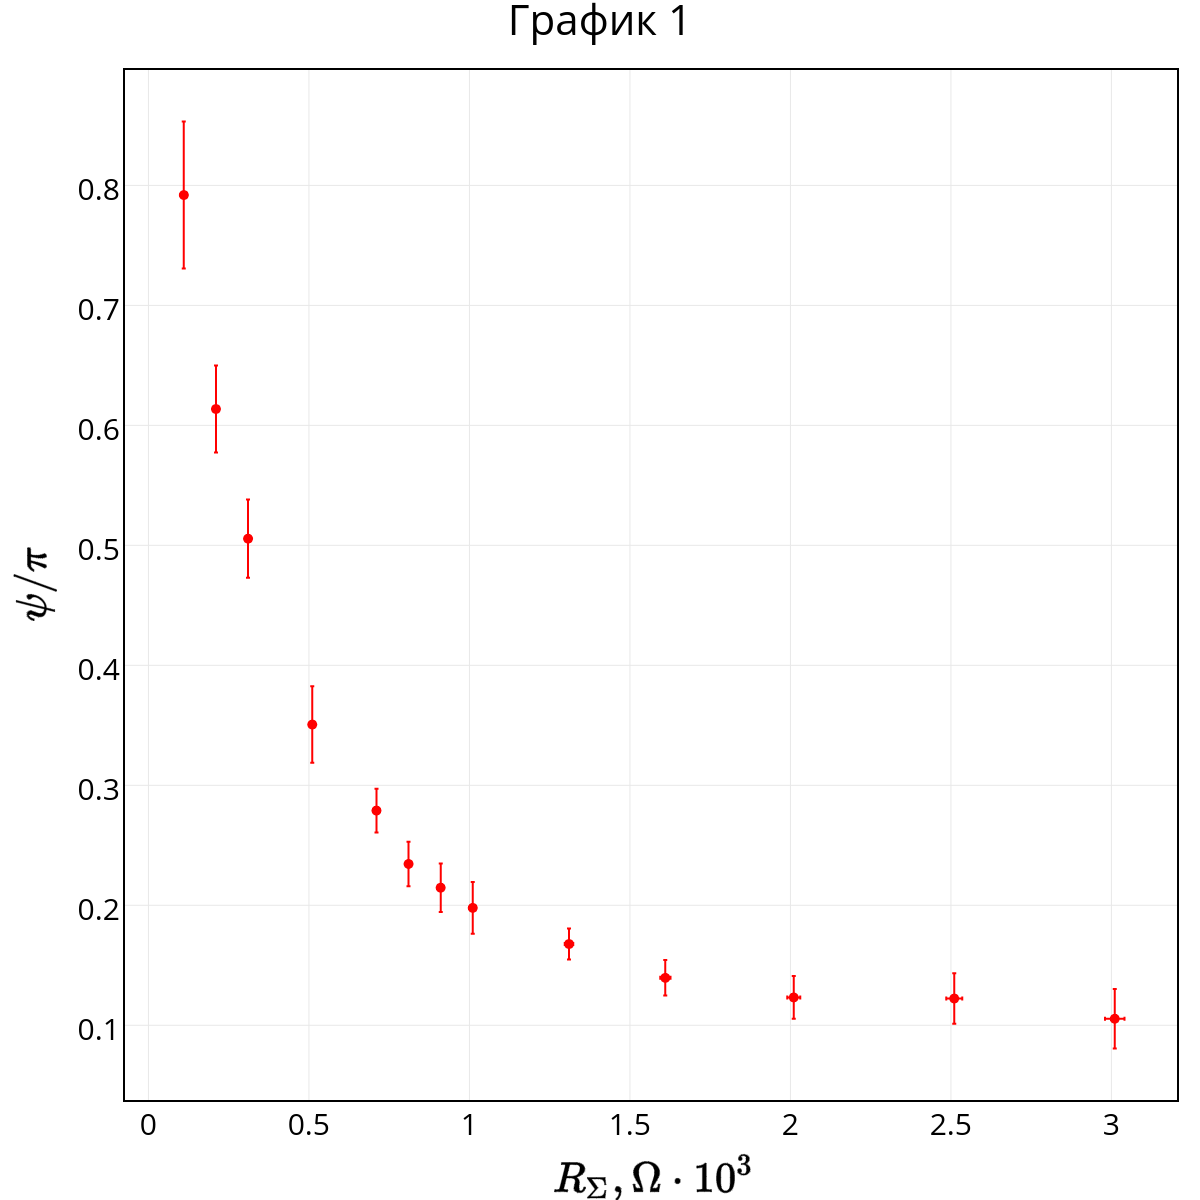
\includegraphics[scale = 0.20]{my_plot1.png}\\

Формализуем задачу и сделаем несколько начальных предположений:

1) Будем предполагать, что истинная модель $y$ линейна, то есть: 
$$ y = X\beta + \epsilon $$
Данное предположение оправдывается визуальным анализом и специфичностью решаемой задачи. 

2) Будем предполагать, что выборка случайна: наблюдения $(x_i,~y_i)$ независимы.
Данное предположение оправдывается возвращением экспериментальной установки в исходное положение, а именно закорачиванием пластин конденсатора и фиксированием арретира.

3) Матрица признаков $X$ является матрицей полного ранга. \\

4) Будем предполагать и далее проверим, что ошибка в измерениях $\epsilon$ случайна
$$ \mathds{E}(\epsilon | x) = 0$$

Основываясь на этих предположениях уже можно показать несмещённость и состоятельность оценки параметра $\beta$. Исходя из этого решим задачу простейшим методом наименьших квадратов (least squares), где решение представимо в виде: 
$$ \beta^{'}=(X^T X)^{-1}X^T y $$
В итоге получим:
$$ \beta = 9,91 \times 10^7 \ V^2 \cdot m^{-1} \cdot kg^{-1} \cdot s^2$$\\

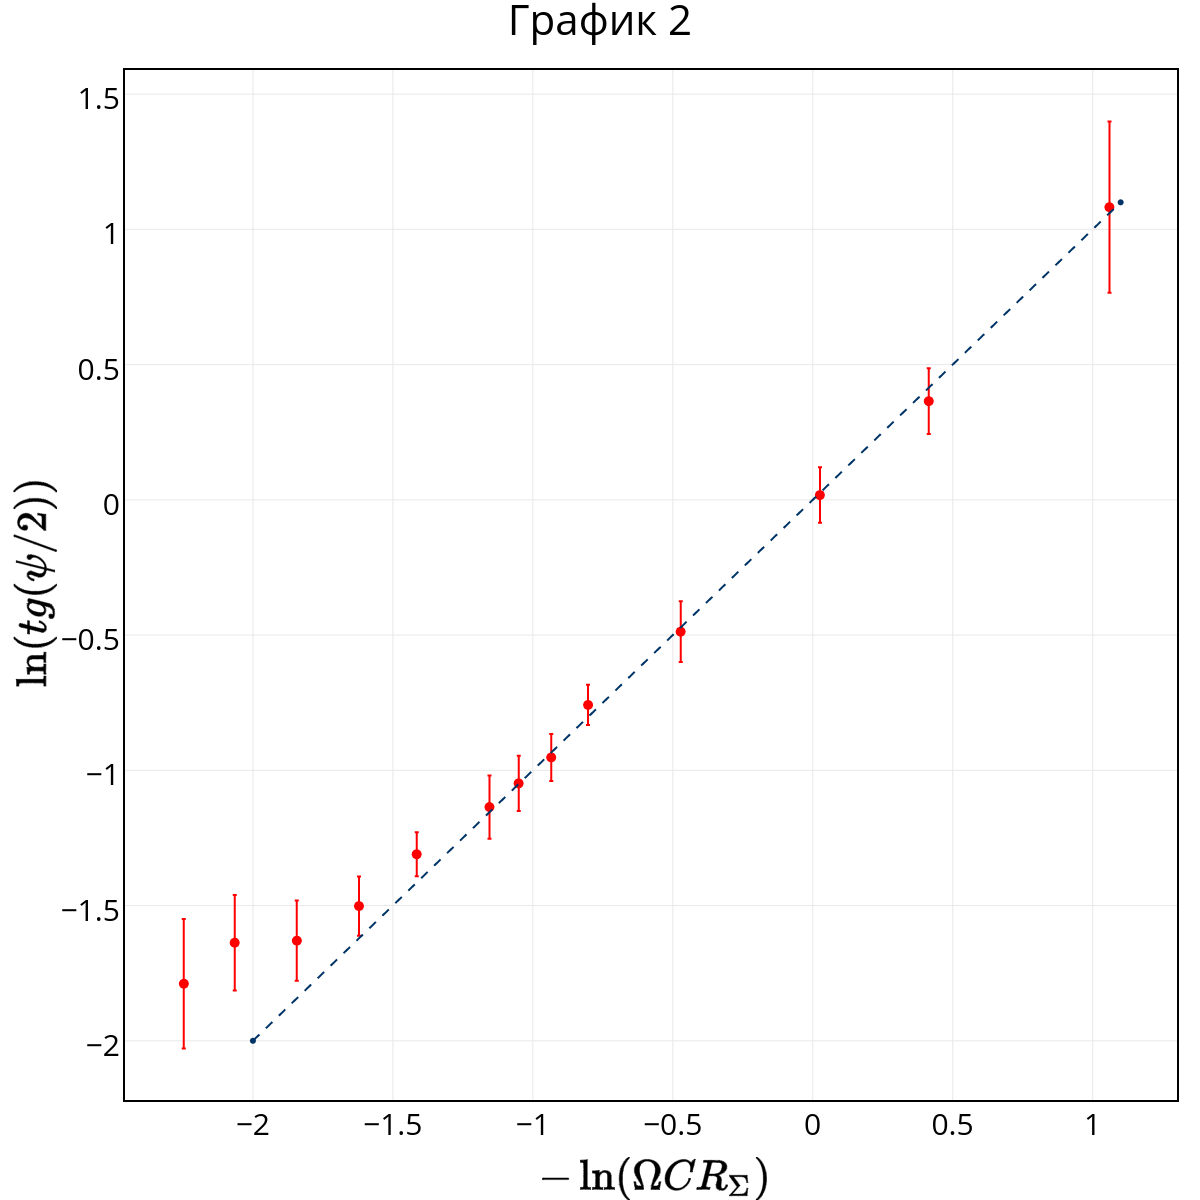
\includegraphics[scale = 0.20]{my_plot2.png}\\

Основываясь уже на этом значении можно дать оценку для $\epsilon_0$:
$$ \epsilon_0 = \frac{2d^2}{S} \beta^{-1} = 12,3 \times 10^{-12} \ F \cdot m^{-1} $$

Продолжим рассматривать предположения о решаемой задаче:

5) Не будем предпологать, что ошибки являются гомоскедастичными. Визуальный анализ по графику gr.2 не позволяет отвергнуть предположение о гомоскедастичности, однако данная гипотеза может быть проверена более формально по критерию согласия Пирсона $\chi^2$ или более статистически мощным критерием Бройша-Пагана. В нашем же случае, предполагая заранее гетероскедастичность, далее будем строить модели со взвешенной ошибкой (weighted least squares).

6) Нормальное распределение ошибки. 
$$ \epsilon|x \sim N(0, \sigma^2) $$ 
Проверку данного предположения также опустим, что остаётся на совести автора и сразу воспользуемся свойствами задачи с данными предположениями. А именно свойством вычисления дисперсии и построения доверительных интервалов для $\beta$: 
$$ \mathds{D}(\beta_j^{'})= \frac{\sigma^2}{(TSS_j)(1-R_j^2)},~~\text{где}$$
$$ TSS_j = \sum_i^n (x_{ij}- \overline{x}_i)^2,~~~~R^2_j=\frac{\sum_i^n (y_i^{'}-\overline{y})}{\sum_i^n (y_i-\overline{y})} $$

Теперь зная как определить дисперсию параметров модели снова построим метод наименьших квадратов и  вычислим ошибки для $\beta$ и $\epsilon_0$:

$$ \beta = 9,9 \times 10^7 \ V^2 \cdot m^{-1} \cdot kg^{-1} \cdot s^2$$
$$ \sigma_\beta^{stat} = 1.8 \times 10^7 \ V^2 \cdot m^{-1} \cdot kg^{-1} \cdot s^2$$
$$ \epsilon_0 = \frac{2d^2}{S} \beta^{-1} = (12,3 \pm 1,8) \times 10^{-12} \ F \cdot m^{-1} $$
Здесь уже учтена и систематическая ошибка при измерении $S$ и $d$. \\

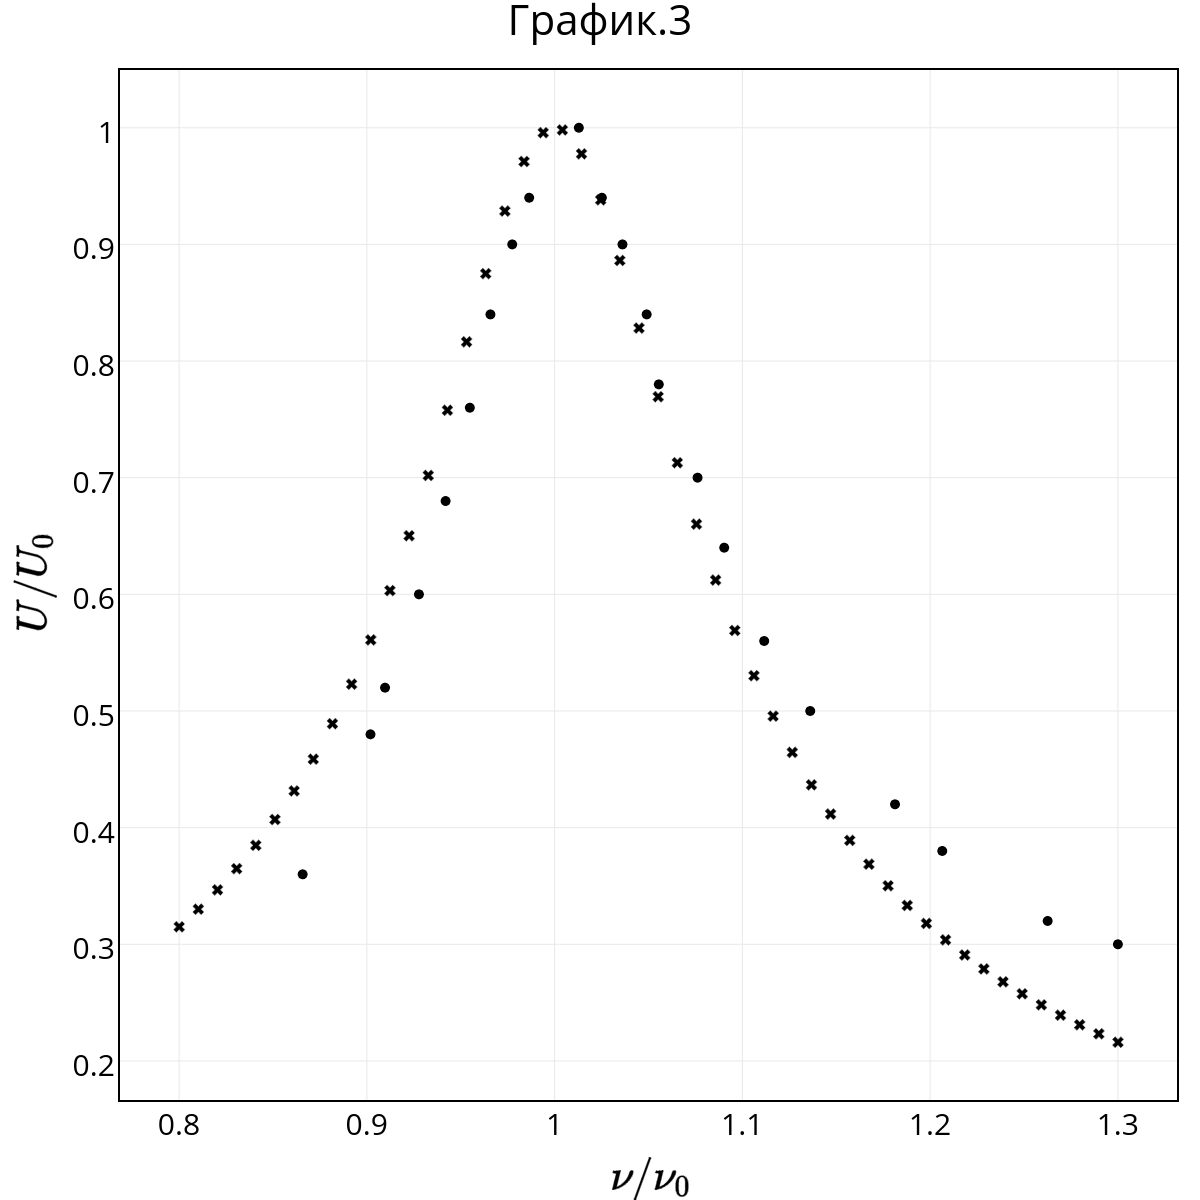
\includegraphics[scale = 0.20]{my_plot3.png}\\

Продолжая анализ эксперимента проверим предположение 4).
Для этого вычислим значения ошибки на каждом элементе выборки и построим график $\epsilon(x)$ (в таблице приведён вариационный ряд по $F$): 

\begin{center}
\begin{tabular}{|c|*{11}{c|}}
\hline
{$\epsilon \times 10^{3} \ V^2$} & $3,5$ &  $3,6$ & $-24$ & $4,3$ & $2,9$ & $7,8$ & $5,5$ & $6,3$ & $38$ & $17$ & $-51$ \\
\hline
\end{tabular}
\end{center}

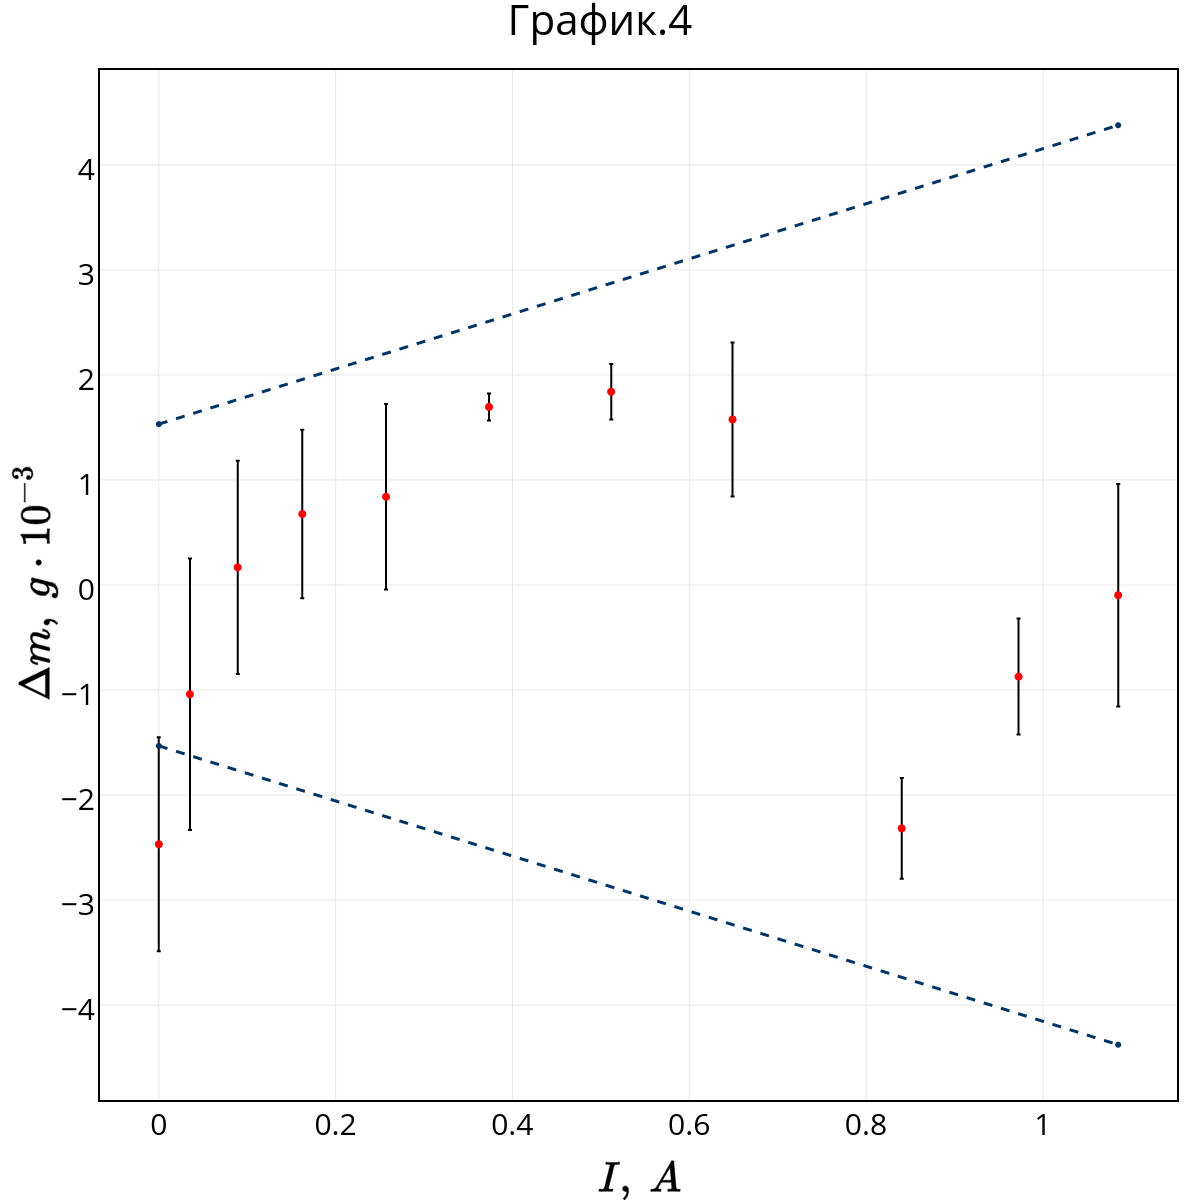
\includegraphics[scale = 0.20]{my_plot4.png}\\

Легко заметить, что мы не совсем хорошо описываем модель. Профиль ошибки отклика сильно смещён в положительную сторону. Также легко заметить, что принадлежность последнего измерения к исходному распределению ошибки отвергается двухвыборочным Z-критерием Стьюдента против двусторонней альтернативы на доверительном уровне значимости $p\approx 0,05$. Это позволяет нам продолжить построение модели без данного измерения. Стоит также заметить, что для двух выкинутых на начальном измерений измерений можно сделать разные выводы. Только гипотеза о принадлежности второго измерения уверенно опровергается аналогичным Z-критерием. 

Проверим гипотезу ($H_0:~\mathds{E}(\epsilon | x) = 0$) по остаткам одновыборочным T-критерием Стьюдента против двусторонней альтернативы ($H_1:~\mathds{E} (\epsilon | x) = 0$).
Получим достигаемый уровень значимости $p_{\text{value}} = 0.2$. Нулевая гипотеза опровергнута быть не может, доверительный уровень значимости для $\mathds{E}(\epsilon | x)$ равен $(-2882, 16108)$.

6) Проверим гипотезу ($H_0:~\epsilon |x \sim N(0, \sigma^2) $) против альтернативы ($H_1:~\text{иначе}$) критерием Шапиро-Уилка.
На десяти измерениях нулевая гипотеза отвергается на доверительном уровне значимости $p_{\text{value}} = 0.04$, ошибки распределены не нормально т.к. сушествуют слишком большие и частые (для данного размера выборки) отклонения от математического ожидания.
Однако, на семи измерениях с самым маленьким отклонением, а именно без третьего и двух последних, нулевая гипотеза опровергнута быть не может на уровне значимости $p_{\text{value}} = 0.55$. Далее проделаем анализ и получим результат на двух вариациях выборки, одна из которых будет без этих 
трёх измерений.

\section{\label{sec:level1}Построение моделей.}
1) Метод наименьших квадратов (least squares):
$$ \beta = \text{argmin}_{\beta}(\sum_i^n (y_i - \beta x_i)^2) $$
2) Взвешенный метод наименьших квадратов (weighted least squares):
$$ \beta = \text{argmin}_{\beta}(\sum_i^n (y_i - \beta x_i)^2 \frac{1}{\sigma_i^2}) $$
3) Orthogonal distance regression (метод учитывающий систематическую ошибку по оси измерения $x$): 
$$ \beta = \text{argmin}_{\beta}(\sum_i^n ((y_i - \beta x_i)^2 + (\frac{y_i}{\beta}-x_i)^2)\frac{1}{\sigma_i^2}) $$

Результат построения выглядит так (индексы $_1$ и $_2$ обозначают выборки до и после критерия Шапиро-Уилка):

\begin{center}
\begin{tabular}{|c|*{3}{c|}}
\hline
{} & $\beta \times 10^7 \ V^2 \cdot m^{-1} \cdot kg^{-1} \cdot s^2$ & $\sigma_{\beta} \times 10^7 \ \text{dim}(\beta)$ \\
\hline
{$\text{ls}_1$} & $10,2$ & $1,2$ \\
\hline
{$\text{ls}_2$} & $10,0$ & $0,2$ \\
\hline
{$\text{wls}_1$} & $10,1$ & $1,6$ \\
\hline
{$\text{wls}_2$} & $10,1$ & $0,4$ \\
\hline
{$\text{odr}_1$} & $10,1$ & $1,7$ \\
\hline
{$\text{odr}_2$} & $10,1$ & $0,4$ \\
\hline
\end{tabular}
\end{center}

\section{\label{sec:level1}Результат.}

По построенным моделям получим значения $\epsilon_0$ и его ошибкой. Усредним значение и ошибку по двум выборкам и по wls и odr:

\begin{center}
\begin{tabular}{|c|*{3}{c|}}
\hline
{} & $\epsilon_0 \times 10^{-12} \ F \cdot m^{-1}$ & $\sigma_{\epsilon_0} \times 10^{-12} \ F \cdot m^{-1} $ \\
\hline
{$\text{ls}_1$} & $11,9$ & $1,9$\\
\hline
{$\text{ls}_2$} & $12,0$ & $1,8$ \\
\hline
{$\text{wls}_1$} & $12,0$ & $1,8$\\
\hline
{$\text{wls}_2$} & $12,0$ & $1,8$ \\
\hline
{$\text{odr}_1$} & $12,0$ & $1,8$ \\
\hline
{$\text{odr}_2$} & $12,0$ & $1,8$ \\
\hline
\end{tabular}
\end{center}

$$\boxed{\epsilon_0 = (12,0 \pm 1,8) \times 10^{-12} \ F \cdot m^{-1}}$$

Табличное значение:

$$\epsilon_0 = 8,854 \times 10^{-12} \ F\cdot m^{-1} $$


\section{\label{sec:level1}СИ vs СГС.}
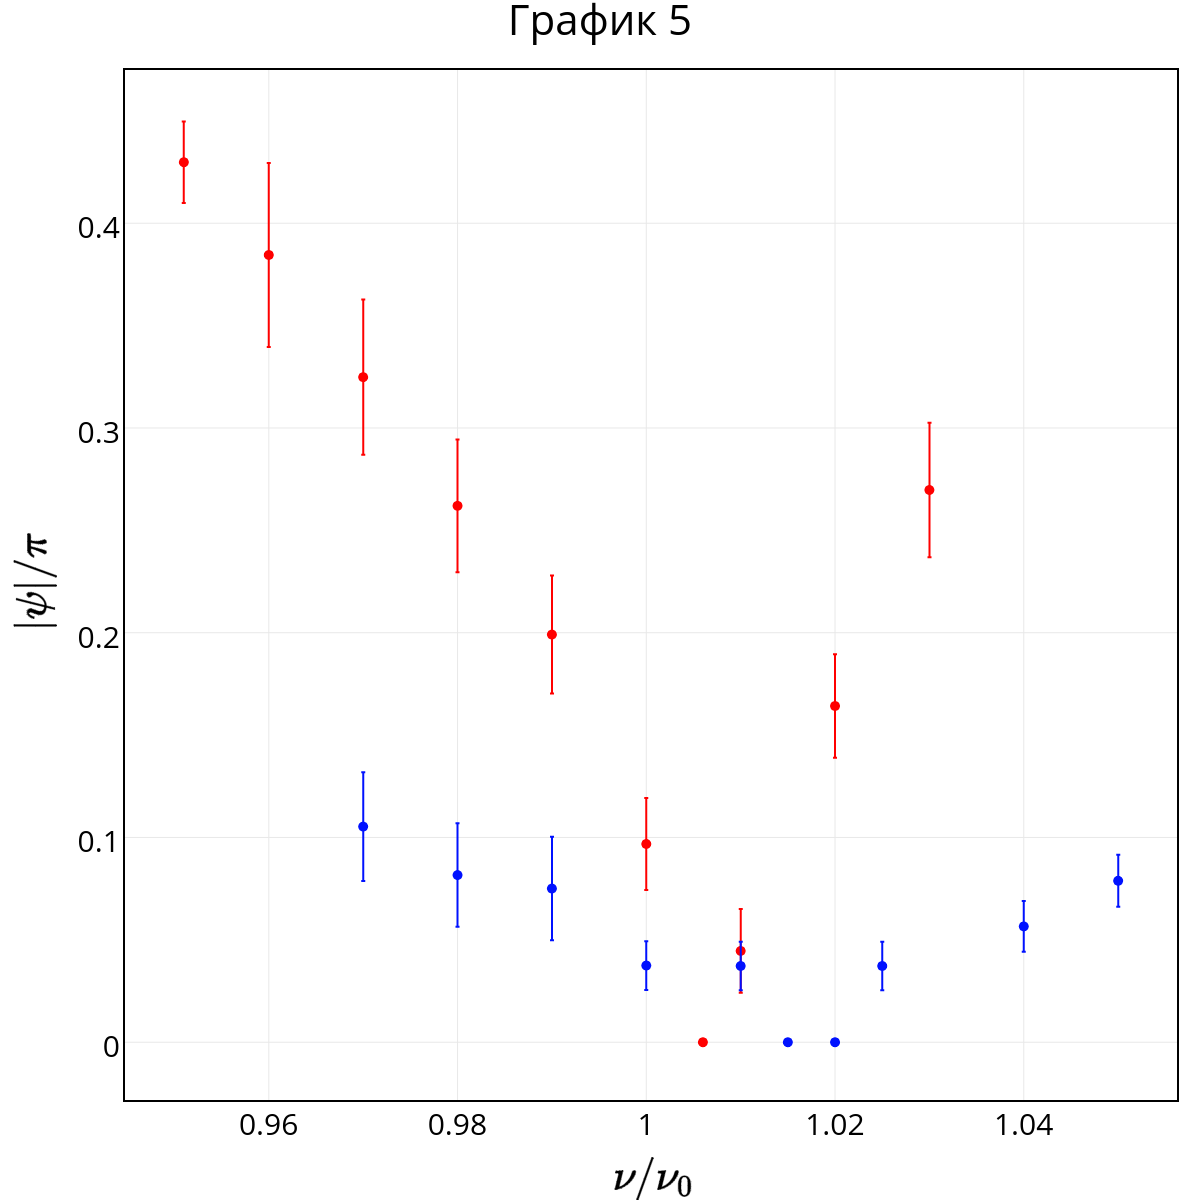
\includegraphics[scale = 0.20]{my_plot5.png}\\

Построим график зависимости посчитанного напряжения с учётом уже полученного значения $\epsilon_0$ в СИ от посчитанного напряжения в системе СГС. \\

Построим взвешенный метод наименьших квадратов (weighted least squares) и получим экспериментальное значение коэффициента перевода единиц напряжения из системы СГС в систему СИ. Учтём ошибки обоих измерений, включая ошибку от нашего значения $\epsilon_0$:

$$\boxed{k = (257 \pm 13) \ V \cdot g^{-1/2} \cdot cm^{-1/2} \cdot s}$$

\section{\label{sec:level1}Ссылки.}

Критерий Стьюдента - scipy.stats.ttest\_1samp

Критерий Шапиро-Уилка - scipy.stats.shapiro

LS and WLS - scipy.optimize.curve\_fit

ODR - scipy.odr

Весь процесс обработки данных можно проделать в открытом репозитории:

\href{github.com/heyfaraday/labs_3sem/tree/master/3.1.2}{github.com/heyfaraday/labs\_3sem/tree/master/3.1.2}
\end{document}
